\documentclass[a4paper, 12pt]{article}

% rubber: module bibtex
% rubber: depend ../litteratur.bib

\usepackage[utf8]{inputenc}
\usepackage[T1]{fontenc}
\usepackage[danish]{babel}
\usepackage[bitstream-charter]{mathdesign}
\usepackage{graphicx}
%% \usepackage{float}
%% \usepackage{varioref}
\usepackage{booktabs}
\usepackage[footnotesize,margin=1cm]{caption}
\usepackage{enumitem}
\usepackage{subfig}
\usepackage{url}
\usepackage[draft]{fixme}

\newcommand{\oevelsenr}{4}
\newcommand{\oevelsetitel}{PACT-analyse med interview}
\newcommand{\afleveringsdato}{6. oktober 2011}

\usepackage{fancyhdr}
\fancyhf{}
\fancyhead[L]{\footnotesize Gruppe 61}
\fancyhead[R]{\footnotesize Øvelse \oevelsenr}
\pagestyle{fancy}

\usepackage[style=numeric]{biblatex}
\addbibresource{../litteratur.bib}

\setdescription{
  font=\normalfont\itshape,
  style=sameline,
  leftmargin=\parindent
}

\begin{document}

\begin{titlepage}
\begin{center}

{\large Menneske-datamaskine interaktion}

\vspace{2cm}

\rule{\linewidth}{0.5mm}\\[3mm]

{\LARGE Øvelse \oevelsenr}\\[6mm]
{\Huge \oevelsetitel}

\rule{\linewidth}{0.5mm}

\vfill

{\bf Gruppe 61}\\[3mm]
\begin{tabular}{lr}
  Claus Skou Nielsen & \texttt{ptf992} \\
  Kasper Passov & \texttt{pvx884} \\
  Michael Budde & \texttt{skx295} \\
  Niels Ørbæk Christensen & \texttt{cxr861}
\end{tabular}

\vspace{1cm}

{\bf Afleveringsdato}\\[3mm]
\afleveringsdato

\vfill

\end{center}
\end{titlepage}


\newpage

\tableofcontents

\newpage
\setcounter{page}{1}
\fancyfoot[C]{\thepage}

\section{Fremgangsmåde}
\label{sec:Fremgangsmaade}

Vi har fulgt forslaget om fremgangsmåden som den bliver beskrevet i
opgaveformuleringen. Vi lagde ud med at udføre en tjekliste, som vi kunne bruge
senere til at interviewe brugerne.

Derefter fandt vi på fire kerneopgaver, der dækkede det vigtigste af sidens
funktionalitet. Det ledte os hen til at udføre en prototype, således at alle
kerneopgaverne er dækket af prototypen. Vi valgte at lave en prototype af papir,
da det er langt det letteste at udarbejde i den indledende fase af design.

Desuden sørgede vi for at overholde reglerne for brugsvenligt design, som det er
blevet gennemgået ved forelæsning, samt vores egne forestillinger om, hvad der
er brugervenligt, og hvad der ikke er.

Vi afleverede vores tjekliste, prototype og kerneopgaver til vores instruktor,
og reviderede vores opgave i forhold til de modtagne rettelser.

Derefter satte vi aftaler op med interviewdeltagere, og foretog løbende
interviews i et interval på fire dage. Vi sørgede for at tage noter under hvert
interview, og vælge interviewdeltagere i forskellige målgrupper.

\subsection{Interviews}

Vi starter hvert interview med at informere interviewdeltagerne om, at vi tester
systemet og ikke dem. Derefter spørger vi til deres erfaring med internet og
computere generelt.

Det næste vi så gerne vil finde ud af, er deres forhold til restauranter. Det er
for at finde ud af, om de overhovedet er typen der går på restuarant, og ville
kunne gøre brug af siden.

Så spørger vi ind til de valg de foretager sig når de vælger en restaurant,
hvilke indflydelser de tager seriøst, om de selv ville gøre brug af diverse
funktionalitet på siden, eksempelvis at skrive en anmeldelse selv --
empiri der er vigtig for dem der skal designe vores vurderingshjemmeside. 

Til sidst debriefer vi deltagerne ved at spørge dem om deres generelle
opfattelse af siden, og om de har nogle ting de synes var gode eller dårlige.

\begin{figure}[htbp]
  \centering
  \begin{tabular}{ l l l l l }
    \textbf{Deltager nr.} & \textbf{Køn}   & \textbf{Alder} & \textbf{Titel} &
    \textbf{Interneterfaring} \\
    \midrule
    1            & Kvinde & 21    & Studerende          & Erfaren         \\
    2            & Kvinde & 54    & Civilingeniør       & Lidt erfaren    \\
    3            & Kvinde & 75    & Pensioneret rektor  & Begynder        \\
    4            & Kvinde & 25    & Studerende          & Erfaren         \\
    5            & Mand   & 56    & Officer             & Erfaren         \\
  \end{tabular}
  \caption{En tabel over testpersoner, der har deltaget i forsøget}
  \label{tab:testpersoner}
\end{figure}



\section{PACT-analyse}

\subsection{People}

Brugergrupper:
\begin{itemize}
\item Studerende
\item Forælder
\item Pensionister
\item Karrieremennesker
\item 25--30 årige i et forhold uden børn
\end{itemize}
Brugerne har varierende erfaring på nettet.

\subsection{Activities}

\begin{itemize}
\item Finde en restaurant i nærheden.
\item Se anmeldelser af nærlæggende restauranter.
\item Skrive en anmeldelse af en bestemt restaurant.
\item Give stjerner til en bestemt restaurant.
\end{itemize}

\subsection{Context}

Brugerne der anvender webstedet vil typisk have god tid, men nogle brugere vil
være under tidspres. Webstedet vil primært blive brugt hjemme eller på kontoret.
Brugerne vil typisk bruge siden et par gange om ugen til et par gange om
måneden.

\subsection{Technologies}

Webstedet kræver en internetbrowser der kører på en almindelig computer, tablet
eller smartphone.

\section{Interviewresultater}
\label{sec:Interviewresultater}
\subsection{Brugerens internetfærdigheder}

  Hvad er dine internet-færdigheder? Bruger du internettet ofte?

    Carl: Bruger nettet hver dag. Er internet erfaren.
    Marie: Er vant på nettet. Kender de fleste standarder.  
    Stine: Bruger nettet meget.
    Vibeke: Bruger internettet en hel del. Søge, yndlingssider/favoritsider, mange andre
	    ting. Googler det hun gerne vil finde.


\subsection{Hvor ofte og til hvilken anledninger}

  Hvor tit spiser du ude?
    Carl: Spiser ude en gang om måneden.
    Hanne: en gang hver anden måned.
    Marie: Spiser ude 2 gange om måneden.
    Stine: ca en gang om måneden.
    Vibeke: Spiser ude et par gange om måneden.
    

  I hvilke anledninger spiser du ude?
    Carl: Som regel i speciel anledning.
    Hanne: Ikke altid i specielle anledninger.
    Marie: Sammen med kæreste eller venner. Ikke kun specielle anledninger.
    Vibeke: Ingen bestemte anledninger. Lyst til at spise ude, eller ikke lyst til at lave mad.

\subsection{Brugerens måde at finde restauranter på}

  Hvordan vælger du steder at spise?
    Carl: Finder restauranter på nettet, som oftest.
    Hanne: Gennem venner eller bekendtskaber.
    Marie: Spurgte på facebook for at finde et sted sidst. Ellers anmeldelser fra aviser/internettet. iByen.
    Stine: noget jeg har hørt om, eller læst om, eller nettet. Jeg leder efter via priser, typer og primært beligenhed
    Vibeke: Afhængig af hvor vi er: Hjemme -> nærområde, går sjældent efter de dyre steder.

\subsection{Forventninger til en restaurant}

  Hvad er vigtigt når du vælger en restaurant at spise på?
  Type, kvalitet, pris, lokation eller stemning?
    Carl: Vuderer på de fleste ting. Køkkentype og hvorvidt det ser indbydende ud er vigtigt.
    Hanne: Madens kvalitet er en stor prioritet.
    Marie: Hyggeligt/stemning. Spændende mad, men stadig inden for rimelig pris.
    Stine: Prisen betyder meget i forhold til valg
    Vibeke: Forskelligt, nogle gange vil man have et hurtig måltid og andre gange en oplevelse.

\subsection{Anmeldelser fra aviser/venner/anmeldere}

  Hvad lægger du vægt på i en anmeldelse?
    Carl: Forventer af andmeldelse: Stemning, service, madkvalitet. Helhedsoplevelse.
    Hanne: Maden er i centrum. Ikke stemning eller service.
    Marie: Velskrevne anmeldelser og engagement. 
	   Stemning og service er også vigtigt. Ikke kun kvaliteten af maden.
    Vibeke: Lægger vægt på at anmeldelsen leverer klare oplysninger. Er køkkenet noget for
	    mig?

  Hvor meget betyder anmeldelser fra f. eks. en avis eller hjemmeside?
    Carl: Anmeldelser fra Aviser og lign. betyder ikke noget.
    Hanne: Anmeldelser bruges også til at vælge restaurent.
    Marie: Anmeldelser betyder meget. Hvis det er en side man kan stole på.
    Stine: Det kan gøre udslaget til hvor jeg tager hen, men er ikke altafgørende
    Vibeke: Hvis vi ser en god anmeldelse indenfor overskuelig afstand, kan vi godt sige der
	    spiser vi. Hvis hele familien skal ud at spise, undersøges der på nettet.


\subsection{Generelle forventinger til en restaurantvuderingshjemmeside}

  Hvad ville kunne få dig til at registrere dig som bruger på hjemmesiden?
  Rabatter, anbefalinger eller andet?
    Carl: Rabatter og tilbud ville være grunde til at registrere sig.
    Hanne: Rabatter kan godt lokke. Lige som Politikens Plus-ordning.
    Marie: Rabatter er vigtigt for at kunne registrere. Også brok er en vigtigt grund.
    Vibeke: Det kunne godt være hun har lyst til at oprette sig som bruger (specielle
	    tilbud, rabatter)

  Hvad forventer du at en restaurationsvurderingshjemmeside indeholder?
    Carl: Forventer fra siden: Menuen, prisleje, beliggenhed.
    Hanne: Skulle indeholde: Menu, prisleje. Koncept, hvis der er noget.
    Marie: Forventer overblik over forskellige kriterier. Køkken, pris, beliggenhed.
	   Overskuelighed er vigtigt.
    Stine: En oversigt over resturanter, og vuderinger af dem.
    Vibeke: Vil forvente at den indeholder en beskrivelse af konceptet, hvor ligger
	    restauranten rent prismæssigt.

\subsection{Anmeldelser fra brugere på en restaurantvuderingshjemmeside}

  Hvor vigtig er kommunikation med andre brugere af hjemmesiden?
    Carl: Anmeldelser fra andre brugere kan have betydning.
    Hanne: Ligegyldigt
    Marie: Kommunikation med andre brugere er vigtigt. Vudere andres anmeldelser, 
	   og selv at kunne skrive anmeldelser er essentielt.
    Stine: meget ligeglad med andres anmeldelser, har ikke noget behov for at snakke med andre brugere
    Vibeke: Kommunikation med andre brugere er ikke vigtigt. Mere mund til mund - med
	    rigtige personer.

  Hvor meget betyder anmeldelser fra andre brugere?
    Carl: Anmeldelser fra brugere og vennner betyder noget.
    Hanne: Anmeldelser fra andre brugere er ikke af høj vigtighed.
    Marie: Kan betyde meget hvis de er velskrevne og virker troværdige.
    Stine: Meget ligeglad med andres anmeldelser, har ikke noget behov for at snakke med andre brugere
    Vibeke: Det betyder ikke noget, hvor det er fra. Har ikke været ude for at læse
	    brugerkommentarer/anmeldelse.

  Ville du gøre brug af at kunne tilkendegive din vurdering af en anmeldelse
  og hvorfor?
    Carl: Vigtigt at kunne kommentere/vudere andres anmeldelser. Ville gøre brug af det hvis uenig eller enig.
    Hanne: Skriver ikke ofte kommentarer, eller tilføjer til nettet på anden vis. Tager ikke brugerkommentarer særligt alvorligt.
    Marie: Vil gerne kommentere, hvis man var uening med en anden anmeldelse.
    Vibeke: Ville ikke skrive.

  Hvad ville få dig til at skrive en personlig anmeldelse af en restaurant?
    Carl: Ville godt kunne finde på at skrive en anmeldelse hvis det var en god oplevelse.
    Hanne: Specielt hvis det er en god oplevelse.
    Marie: Enten skide-godt eller skide-dårligt for at gide at skrive en restaurant.
    Vibeke: Hvis jeg bliver meget overrasket, vil jeg skrive en anmeldelse.

\section{Kerneopgaver}
\label{sec:Kerneopgaver}
\begin{itemize}
\item Se reviews af resturanter i et område
\item Se reviews af restauranter for en bestemt køkkentype
\item Find bestemt restaurant og se reviews/kommentare, stjerner
\item Skriv review/kommentar for en bestemt restaurant
\end{itemize}

\section{Målgruppebeskrivelser}
\label{sec:Maalgruppebeskrivelser}

\begin{description}[style=nextline,font=\bf]
  \item[Familier med små børn]

    En familie der alle bor sammen og tager ud at spise i
    fælleskab. De har yngre børn og det er derfor vigtigt for dem at
    stemningen er god og at det er nemt at komme hen til restauranten.

  \item[25--30 årige storby-par uden børn]

    Unge mennesker der har taget en længerevarende uddannelse og har
    fået gode job og derfor har en sund økonomi og overskud i
    hverdagen. De har mange kulturelle interesser og vil gerne prøve
    nye populære restauranter.

  \item[Pensionister]

    Ældre mennesker der nyder at bruge deres pensionsår på at gå ud på
    restauranter og lede efter gode tilbud. De har tid til at
    planlægge deres restaurant-besøg nøje og går efter at få meget
    værdi for pengene.

  \item[Karrieremennesker]

    Mennesker i de sene 30'ere til de tidlige 50'ere der arbejder
    meget og har deres karriere som en top-prioritet. De har luft i
    økonomien, men har ikke megen tid til at lede efter den rigtige
    restaurant som de skal bruge til arbejdsfrokoster eller lignende.

  \item[Studerende]

    Unge personer i 20'erne der uddanner sig i eller omkring
    København. De har ikke særligt mange penge at gøre godt med, og
    pris er derfor vigtigt for dem. De har desuden intet motoriseret
    køretøj og ønsker at finde restauranter i nærheden.
\end{description}

\subsection{Uddybelse af målgruppen \emph{Karrieremennesker}}
Det karriereorienterede menneske går ofte på restuarant, både som privatperson
eller i forretningsøjemed. Personen kan både være mand eller kvinde, men vil
oftest være 30--50 år, og have en god indtjening der giver mulighed for at spise
ofte på restaurant uden at skulle tænke over prisen.

Det karriereorienterede menneske ønsker at finde gode restauranter hurtigt. Det
er vigtigt at restauranterne er gode og præsentable, da de også tit skal bruges
til forretningsfrokoster. Derfor forventer hun at man nemt kan se billeder,
anmeldelser og en beskrivelse af restuarenterne, som hun vil bruge til at
vurdere om de passer til den givne frokost. 

Denne slags bruger vil næste udelukkende benytte sig af at søge og finde
restauranter, fremfor at skrive anmeldelser af restauranter og kommentarer af
andres restauranter. Det er fordi hun ikke ser restuarantbesøgene som ren
fornøjelse. Hendes restaurantbesøg har som regel et formål; enten at underholde
en forretningspartner, eller bare at få et måltid mad når hun ikke selv har
tid/overskud til at lave mad. 

Disse brugere vil næsten altid have ret meget erfaring med internettet, som er
de eneste forudsætninger for at kunne bruge siden effektivt. De vil også bruge
lignende sider til at effektivere andre dele af deres hverdag, som transport,
udlandsrejser eller indkøb.

\section{Personas}
\label{sec:Personas}

\subsection{Christian Olesen}
Christian er 39 år og bor på Østerbro. Han arbejder som key account manager hos
et større forsikringsselskab. En af han primære opgave er at varetage de større
kunders forsikringer og forbedre deres aftaler med firmaet. Dette involverer
ofte forretningsfrokoster hvor man kan diskutere aftalen samtidigt med at kunden
føler sig værdsat i firmaet.

Christian er meget erfaren med computere og internettet. Han bruger computere
meget i løbet af sin arbejdsdag, og bruger også internettet meget i sin
sparsomme fritid. Han handler ofte på nettet, og bruger også nettet ofte til at
finde informationer. 

Christian er enlig og arbejder meget. Han kommer ofte først hjem fra arbejde
efter de lokale butikker har lukket. Han tager derfor ofte ud at spise på
restuaranter i nærheden af hans kontor ved Kongens Nytorv. Siden der er så stor
omskiftning af restauranterne i området finder han gerne en ny restuarant på
internettet der ligger i nærheden og passer til hvad han lige har lyst til.
Foruden hans personlige behov, bruger han også internettet når han skal finde
steder han kan invitere kunder til forretningsfrokost. 

\subsection{Malene Lund Ibsen}
Malene er 23 år og bor på Amager. Hun studerer dansk på Københavns Universitet
har et studiejob på det lokale bibliotek. Hun kan godt lide god mad; både selv
at lave det, men også at spise det på restuarant. Grundet hendes begrænsede
indtægt er det vigtigt for hende at hun får en god oplevelse for hendes penge.
Hun har tid nok til at undersøge hvilken restuarant hun ønsker at besøge inden
hun bruger pengene på det, og bruger internettet meget til at finde steder at
spise.

Hun er erfaren i bruge almindelige programmer på en computer og er meget vant
til at bruge internettet; både til at finde informationer, men også bare til
underholdning og overspringshandlinger. På hendes job bruger hun også computere
til at søge bibliotekernes databaser igennem. 

Malene har en kæreste, og de fejrer ofte specielle datoer i deres fælles
historie ved at gå ud og spise, hvor resturantens stemning og servering er
vigtig for at de får en tilpas romantisk oplevelse.

\section{Scenarier}
\label{sec:Scenarier}

\subsection{Scenarie 1: Christian Olesen har et vigtigt møde}
\label{sub:Scenarie 1: Christian Olesen}
Christian Olesen har en vigtig forretningsaftale. Det betyder meget for
Christian, at kunden har en kort afstand til restauranten som Christian skal
vælge at spise på, så de kan starte forretningsmiddagen på god fod. Derfor
betyder pris heller ikke noget.

Christian vælger at gå ind på siden, for at finde en passende restaurant nær
kundens placering. Han finder de højst vurderede restauranter i kundens
nærområde, uden hensyn til prisen. Han vælger en restaurant med den bedste
vurdering og dyreste pris, finder kontaktinformationen på siden, og ringer og
reserverer plads.

\subsection{Scenarie 2: Malene Lund Ibsen bliver stiktosset}
\label{sub:Scenarie 2: Malene Lund Ibsen}

Hun har spist på en bestemt sushi-restaurant en gang før og har var tilfreds.
Men på hende og hendes kærestes årsdag, hvor de spiser på sushi-restauranten
sammen, finder hun ud af at restauranten har en ret, der næsten indeholder det
samme som den hun bestilte sidste gang, men kun er halvt så dyr.

Det gør at Malene føler sig snydt, hun synes det er fupmageri at restauranten
har to næsten identiske retter, men tager mange flere penge for den ene af
retterne. Derfor går Malene ind på siden, for at skrive en vred anmeldelse.  Hun
finder restauranten, og skriver en vred kommentar på restaurantens side, hvor
hun giver den nul stjerner.
\section{Testresultater fra prototype}
\label{sec:Testresultater fra prototype}

\section{Erfaringer}
\label{sec:Erfaringer}

\clearpage
\appendix

\section{Tjekliste}

Du vil komme til at prøve en tidlig test-udgave (prototype) som ikke vil ligne
det endelige site.
\begin{itemize}
\item Vi tester websitet og konceptet, ikke dig. Det er ikke en
  eksamen. Vi sætter pris på alle dine kommentarer.
\item Hvad er dine internet-færdigheder? Bruger du internettet ofte?
  Har du selv et website?
\end{itemize}

\paragraph{Anledning}
\begin{itemize}
\item Hvor tit spiser du ude?
\item I hvilke anledninger spiser du ude?
\end{itemize}

\paragraph{Brugsmønstre}
\begin{itemize}
\item Hvordan vælger du steder at spise?
\item Hvad er vigtigt når du vælger en restaurant at spise på?
  \begin{itemize}
  \item Type, kvalitet, pris, lokation eller stemning?
  \end{itemize}
\item Hvor meget betyder anmeldelser fra f. eks. en avis eller hjemmeside?
\item Hvor meget betyder anmeldelser fra andre brugere?
\item Hvad forventer du at en restaurationsvurderingshjemmeside indeholder?
\item Hvor vigtig er kommunikation med andre brugere af hjemmesiden?
\item Hvad lægger du vægt på i en anmeldelse?
\item Hvad ville få dig til at skrive en personlig anmeldelse af en restaurant?
\item Hvad ville kunne få dig til at registrere dig som bruger på hjemmesiden?
Rabatter, anbefalinger eller andet?
\item Ville du gøre brug af at kunne tilkendegive din vurdering af en anmeldelse
og hvorfor?
\end{itemize}

\paragraph{Debriefing}
\begin{itemize}
\item Hvad synes du om webstedet?
\item Hvilke 2--3 ting fungerer bedst på webstedet?
\item Hvilke 2--3 ting trænger mest til at blive forbedret?
\end{itemize}

\section{Prototype}

\begin{figure}[hp]
  \centering
  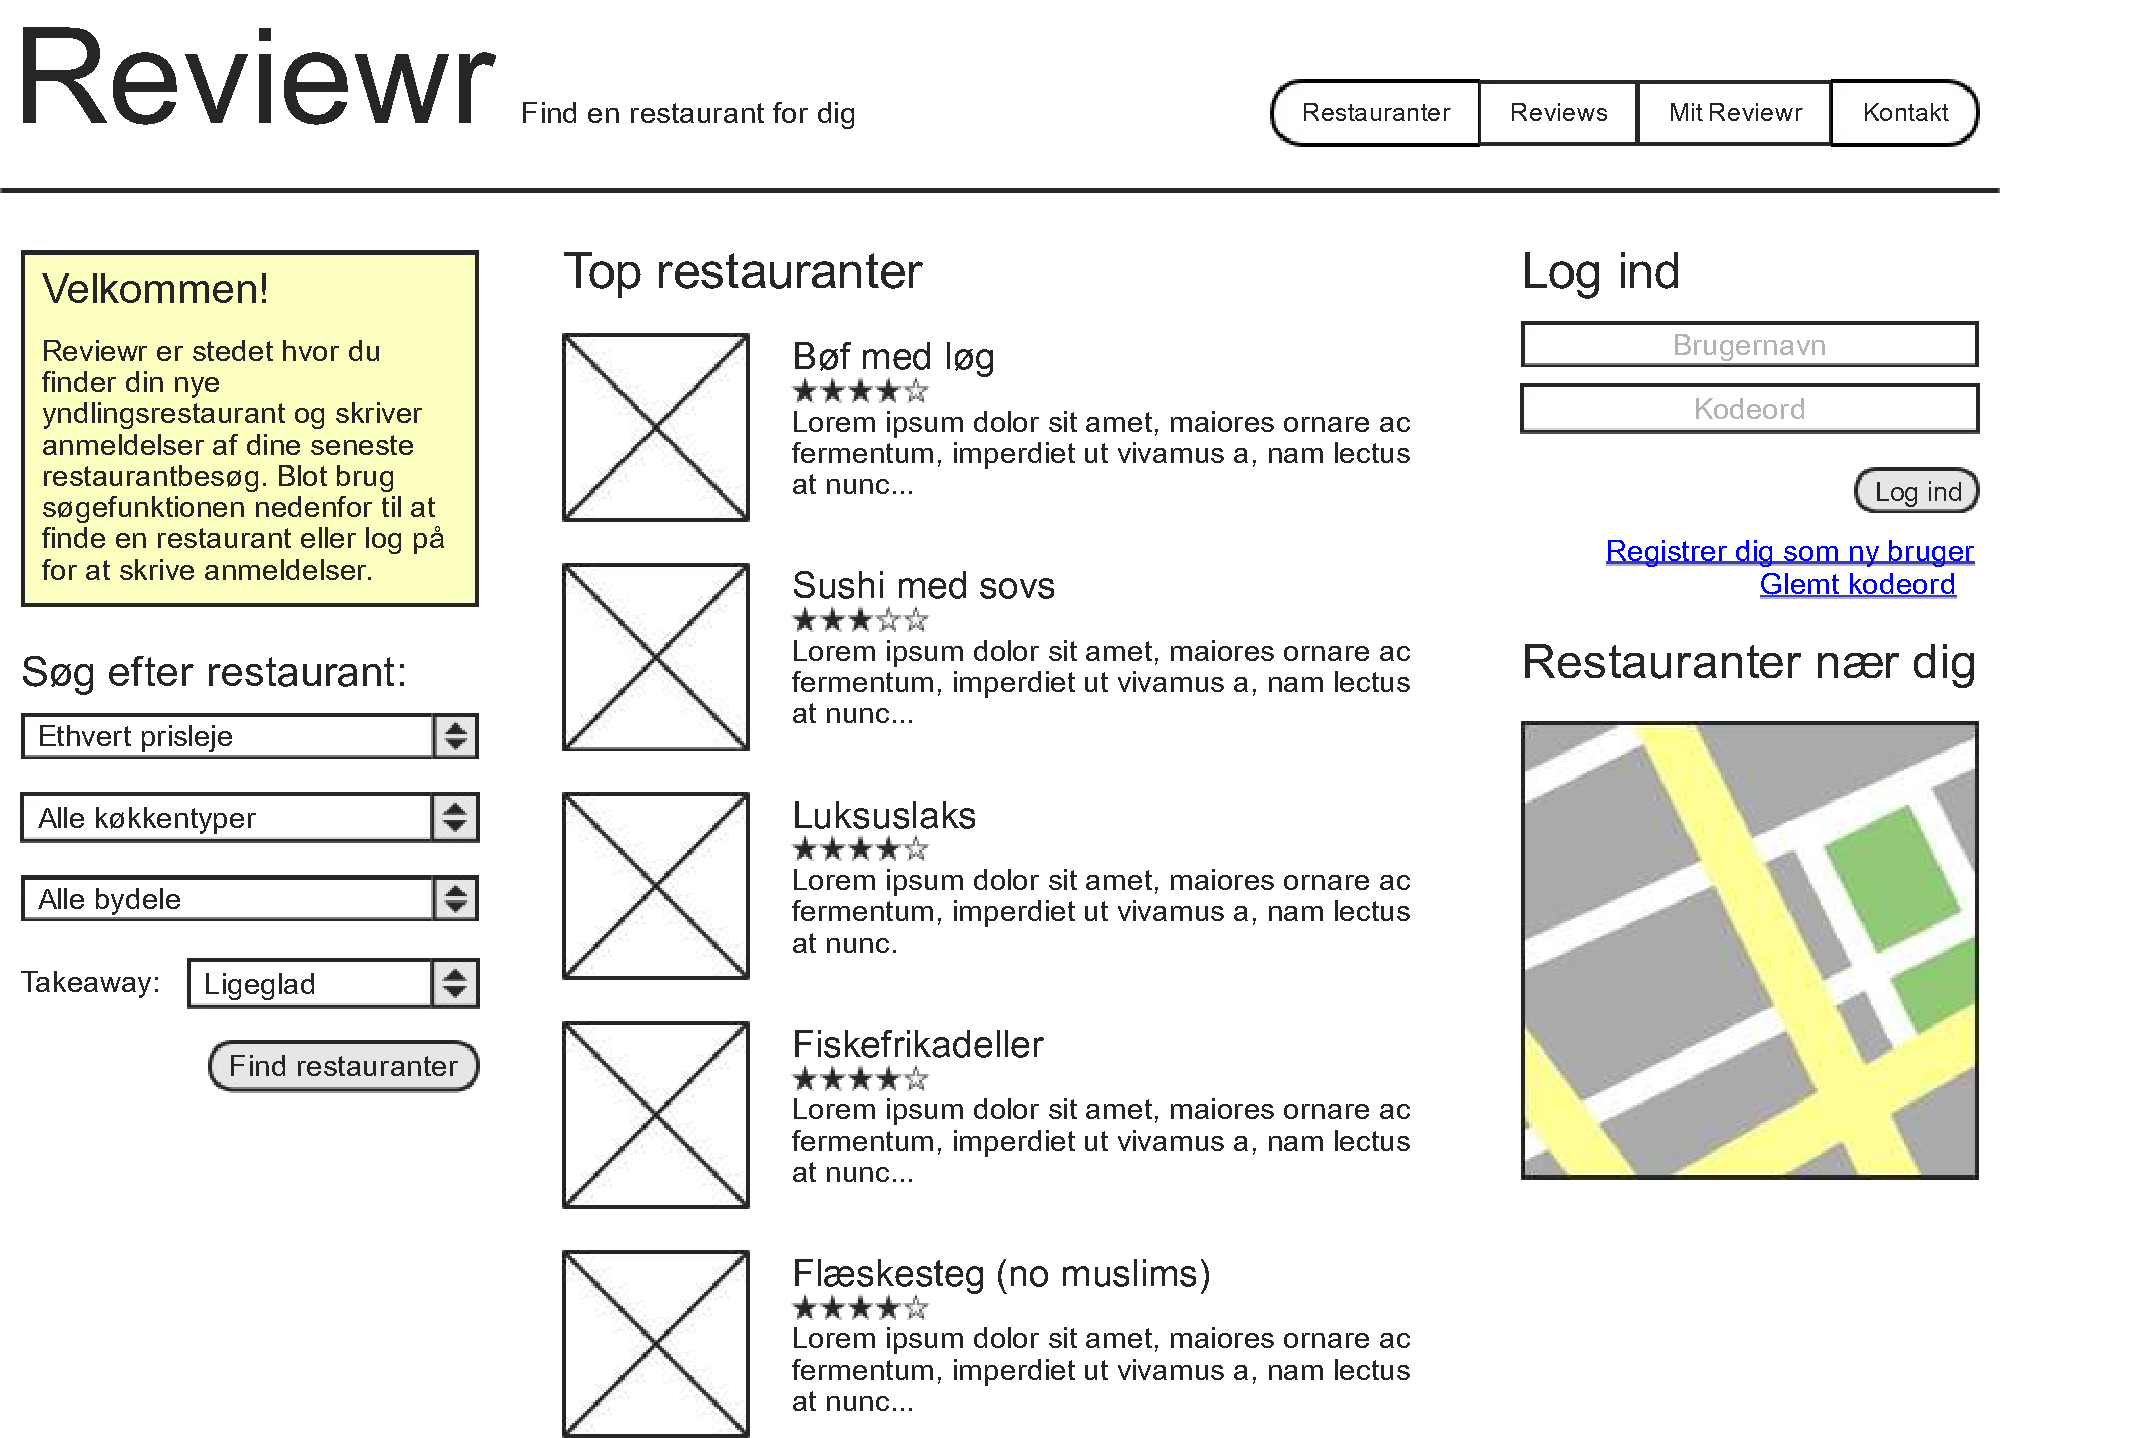
\includegraphics[width=0.9\textwidth]{mockup/page1.pdf}
  \caption{Forsiden for vores prototype.}
\end{figure}

\begin{figure}[hp]
  \centering
  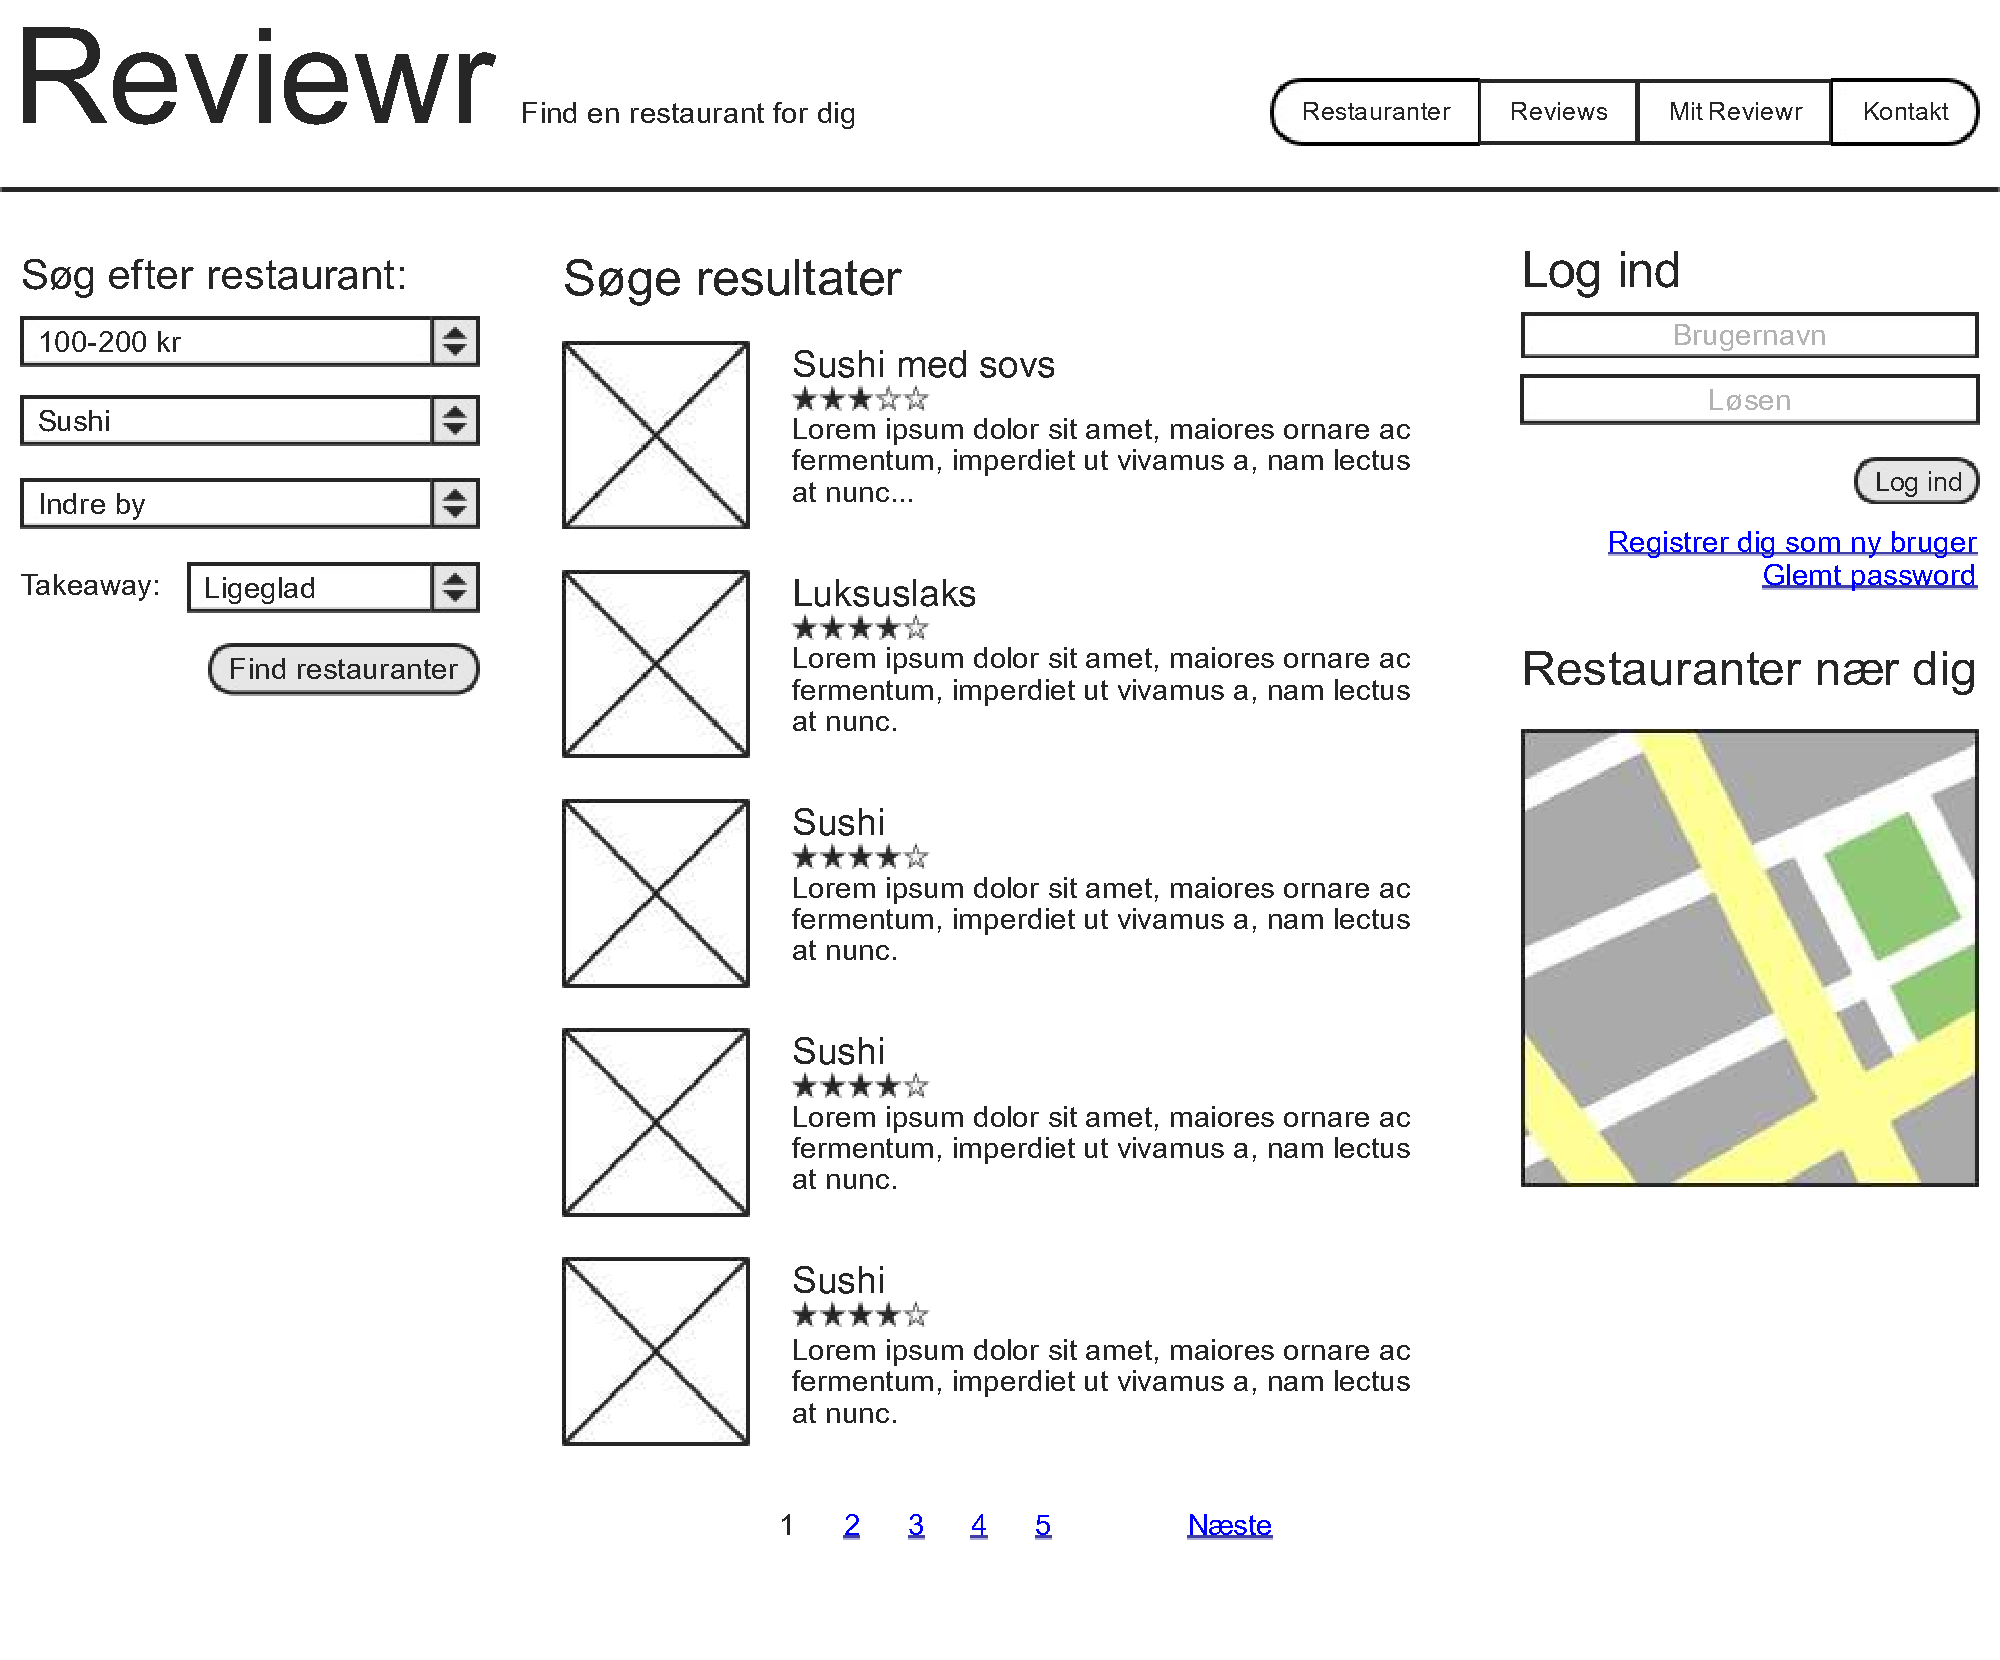
\includegraphics[width=0.9\textwidth]{mockup/page2.pdf}
  \caption{Siden der vises når man søger på restauranter ved hjælp af
    søgefunktionaliteten på forsiden.}
\end{figure}

\begin{figure}[hp]
  \centering
  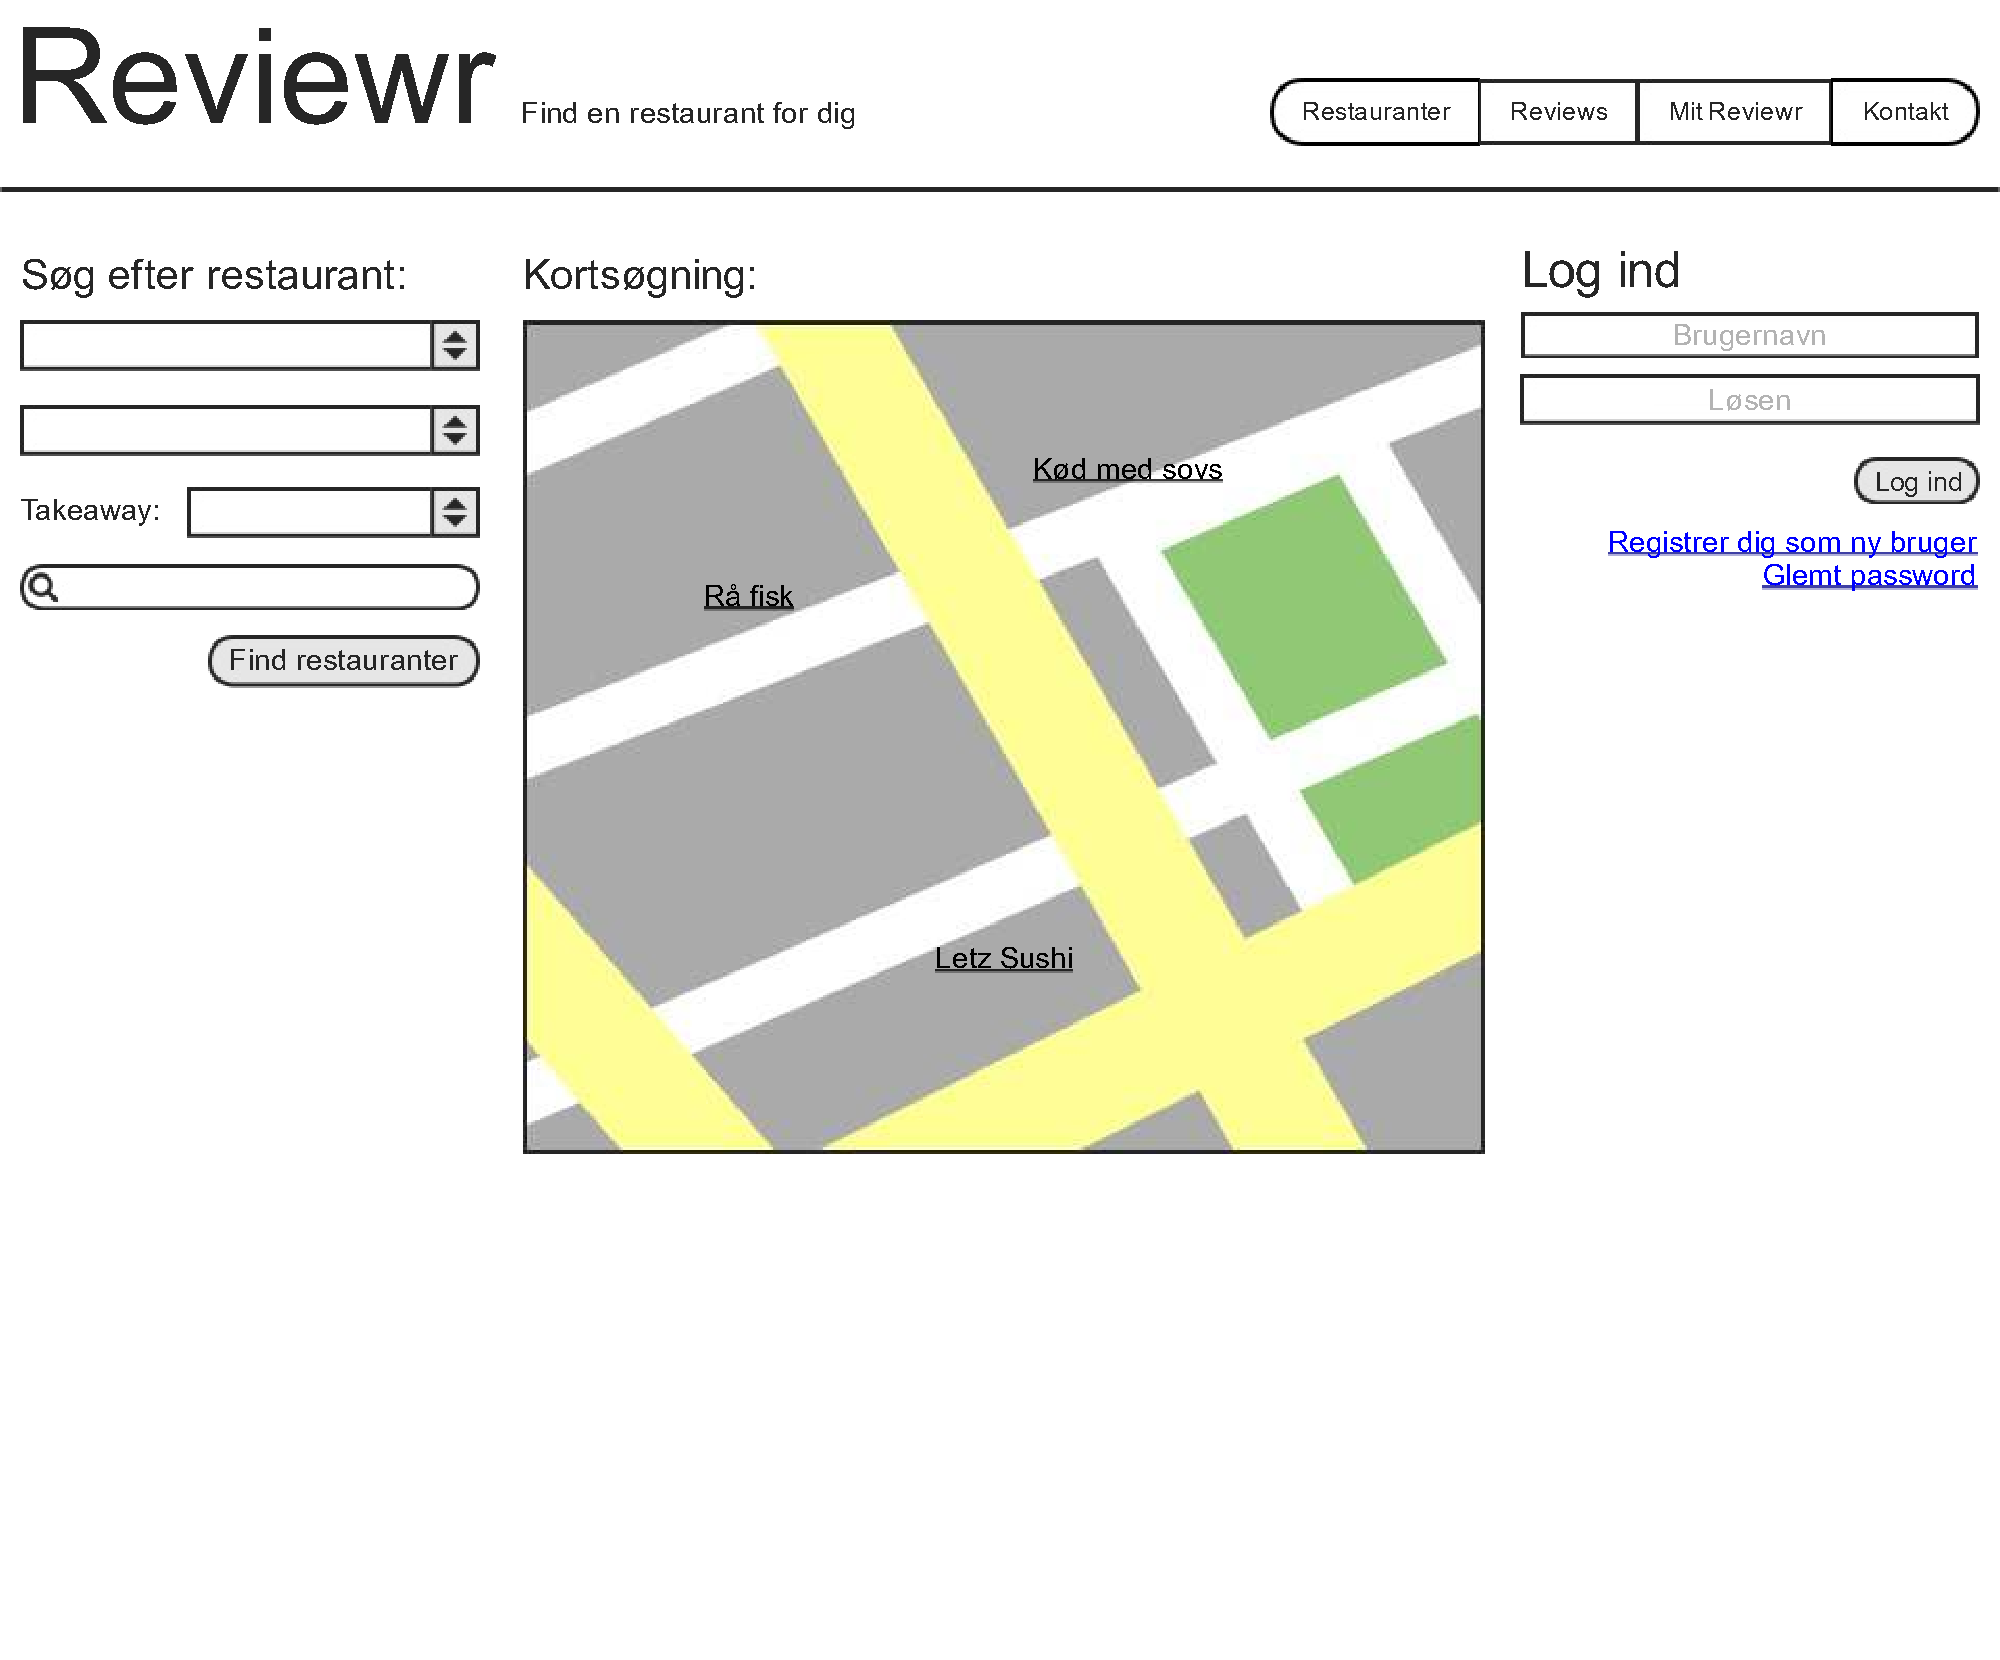
\includegraphics[width=0.9\textwidth]{mockup/page7.pdf}
  \caption{Siden der vises man klikker på det lille kort på forsiden.}
\end{figure}


\begin{figure}[hp]
  \centering
  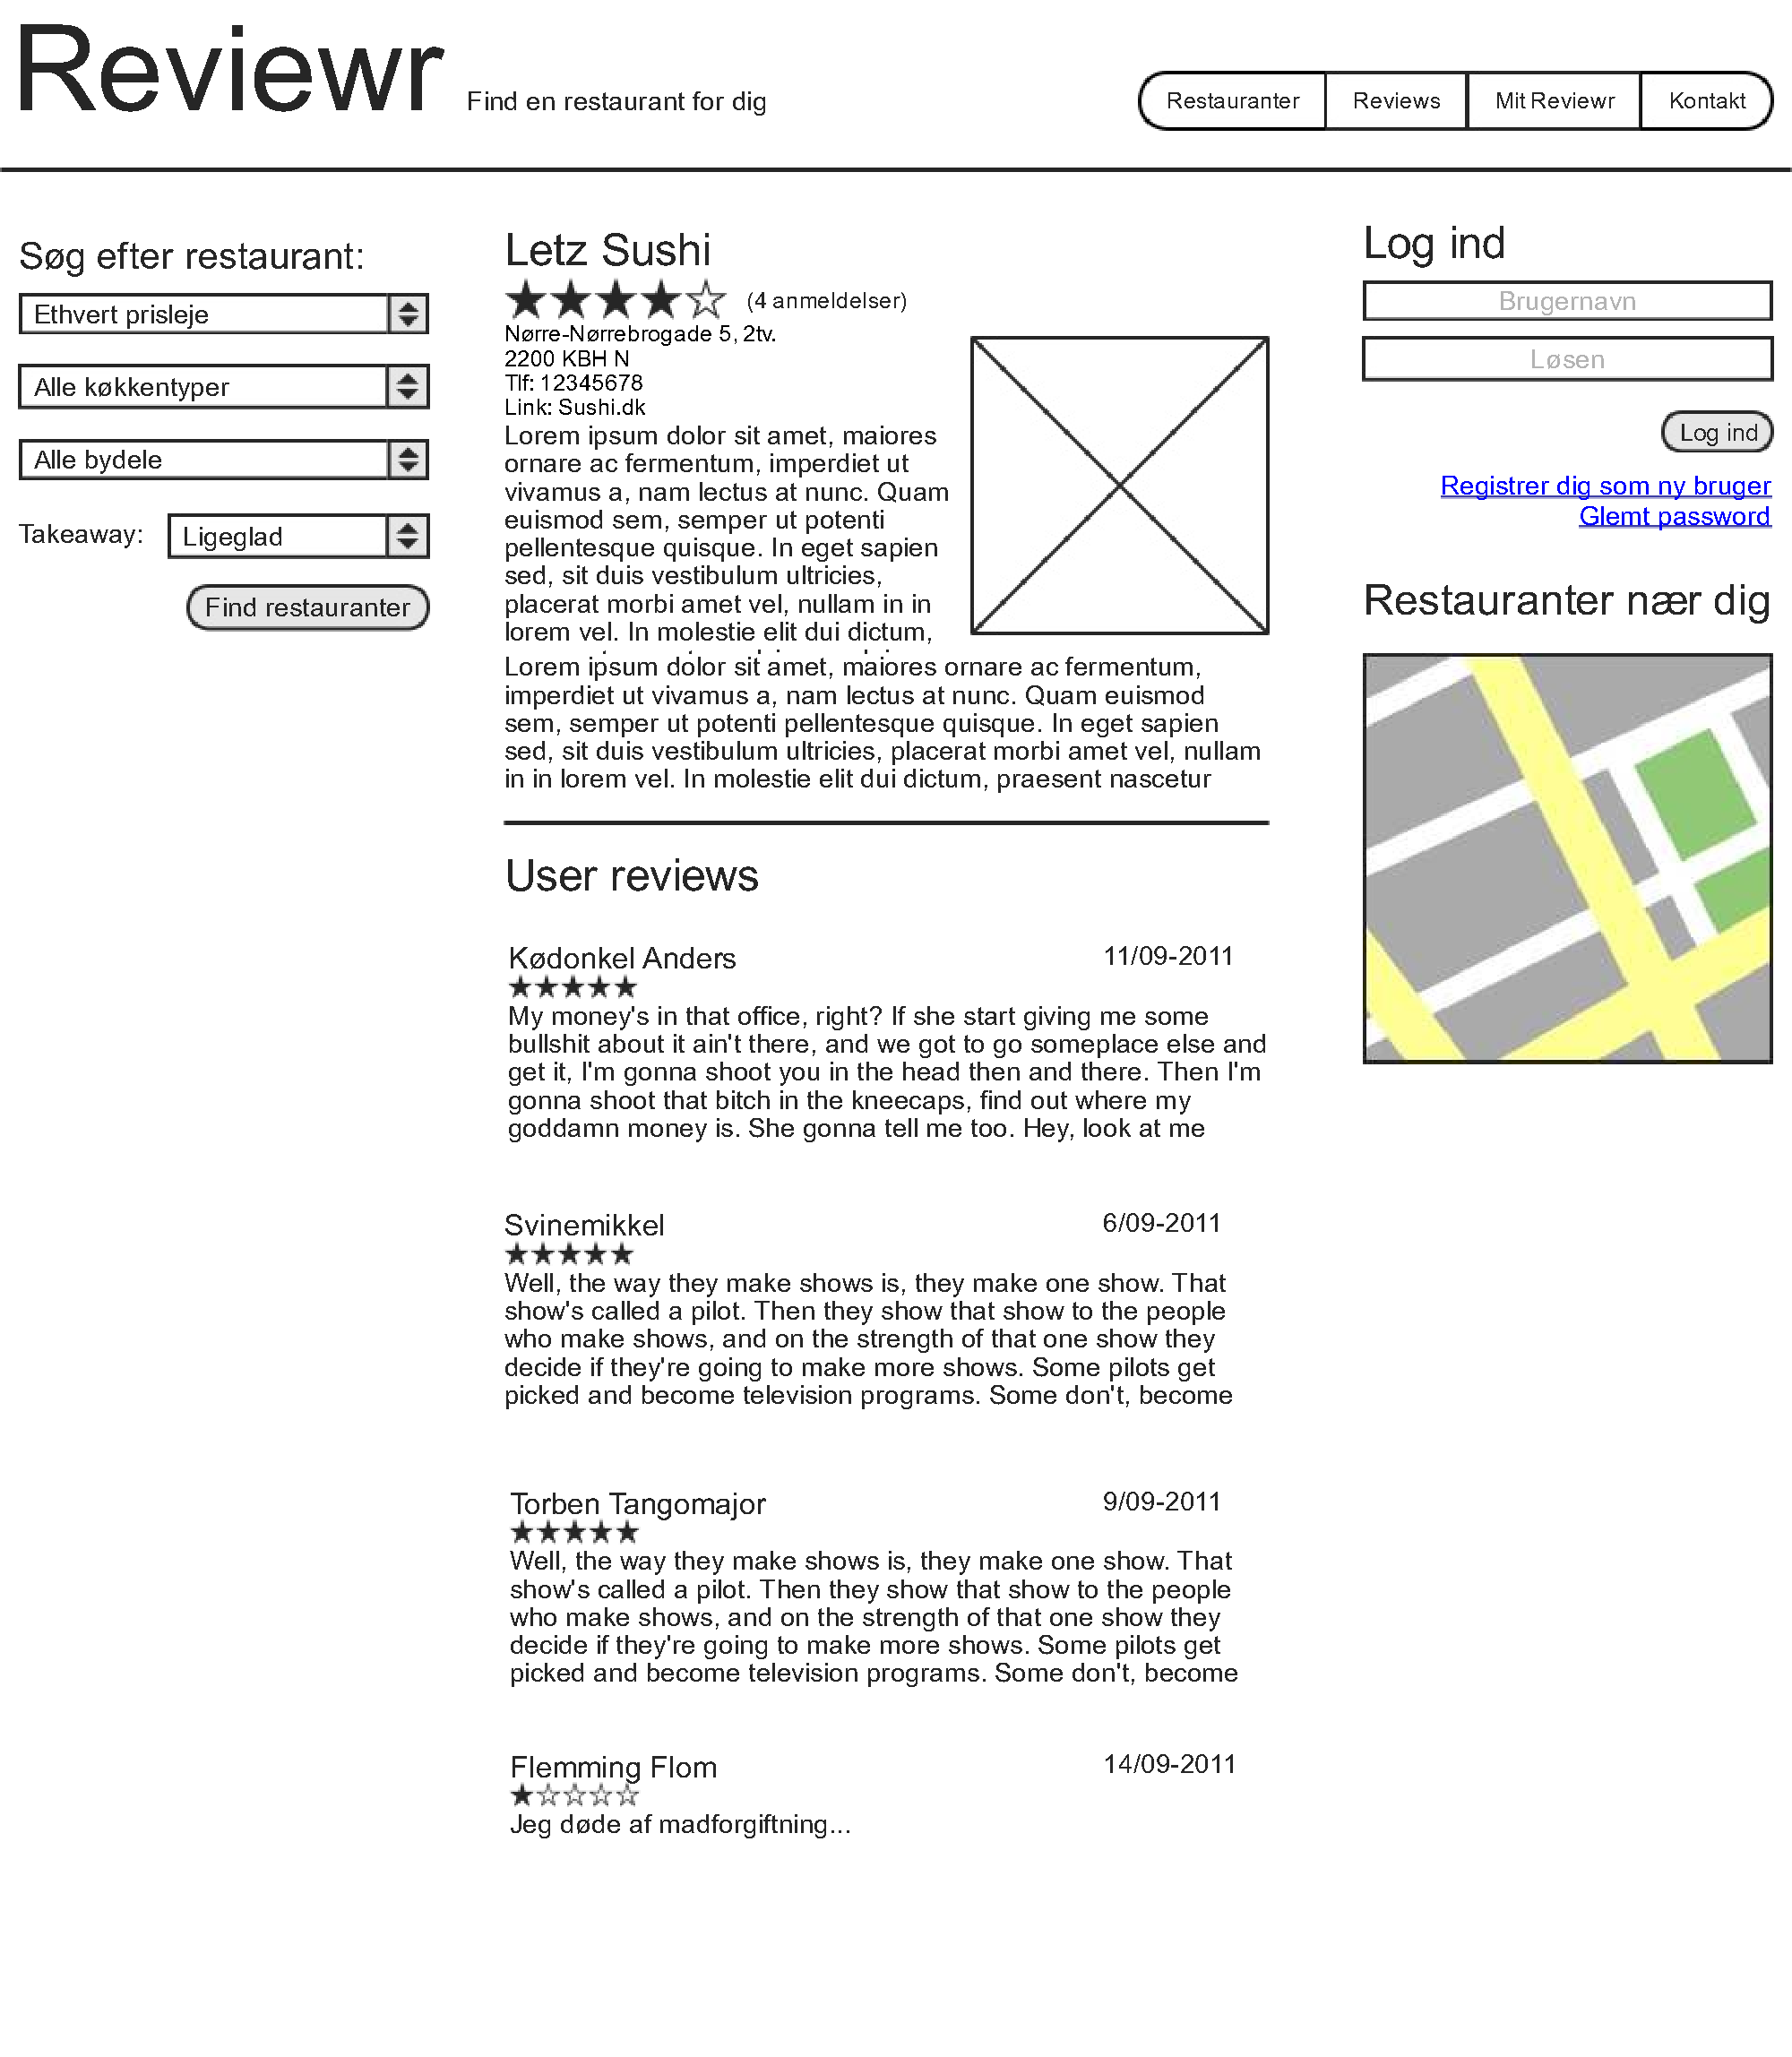
\includegraphics[width=0.9\textwidth]{mockup/page3.pdf}
  \caption{Siden for en enkelt restaurant.}
\end{figure}

\begin{figure}[hp]
  \centering
  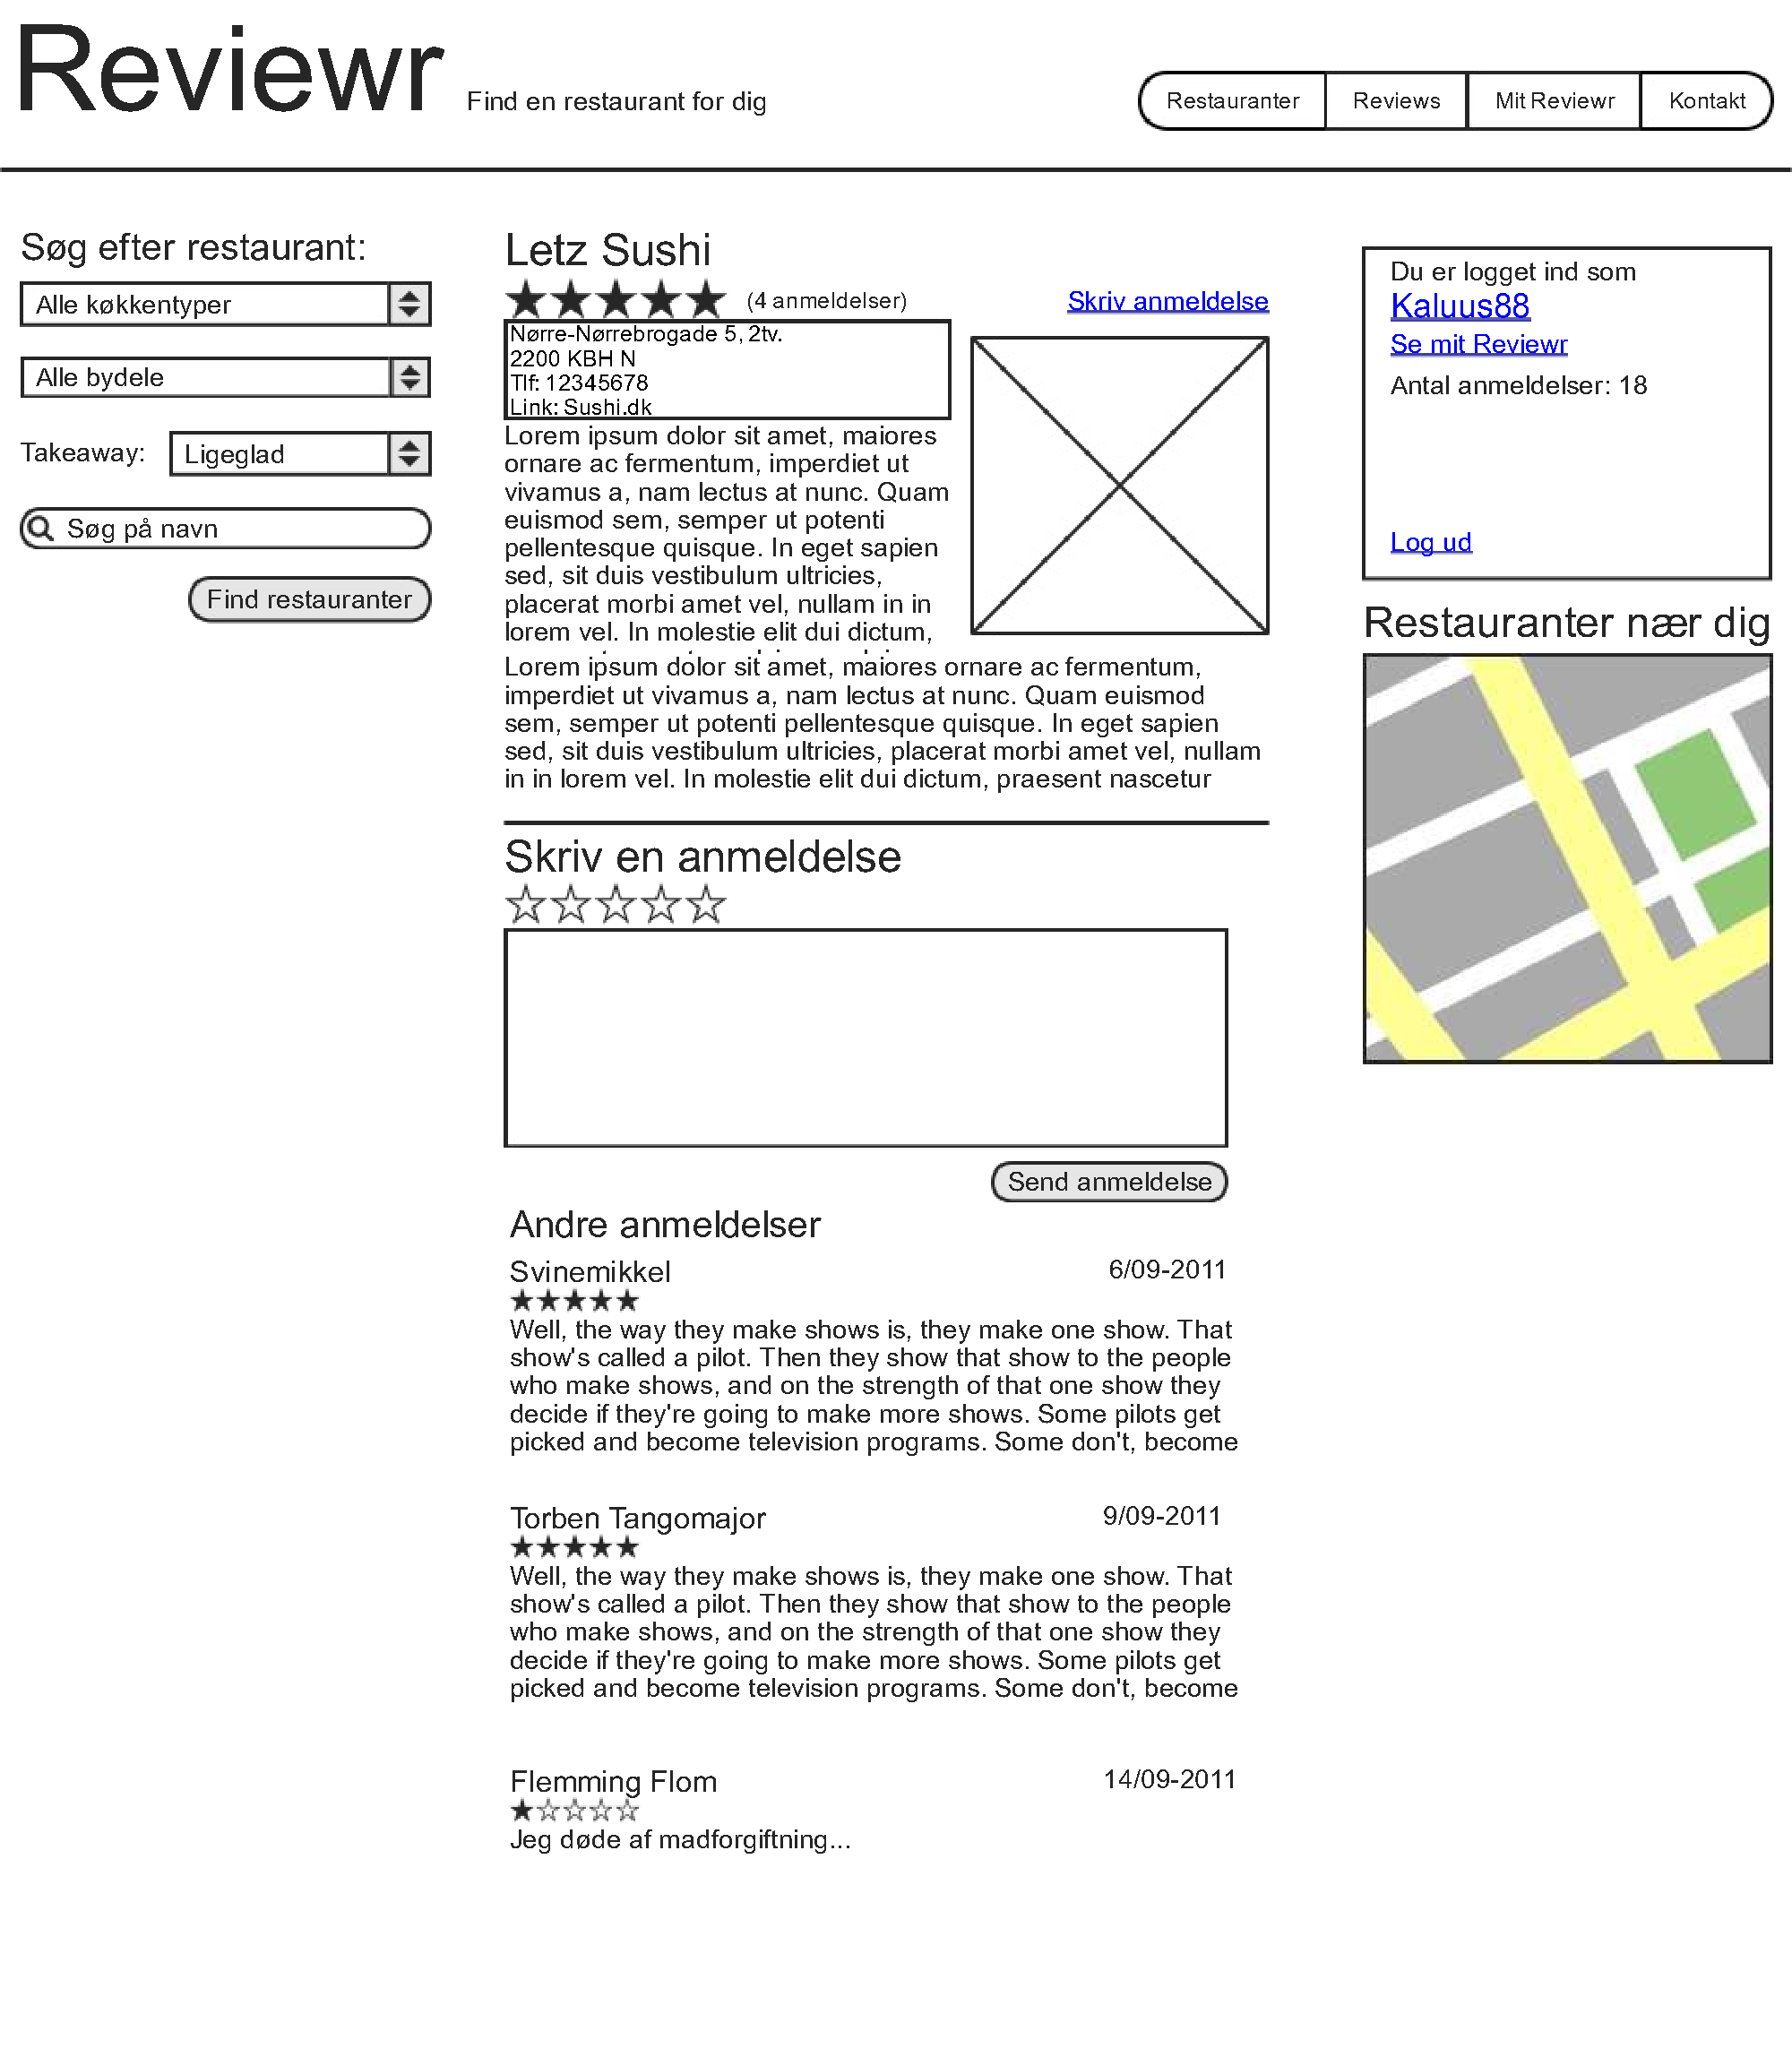
\includegraphics[width=0.9\textwidth]{mockup/page6.pdf}
  \caption{Siden for en enkelt restaurant når man er logget ind.}
\end{figure}

\begin{figure}[hp]
  \centering
  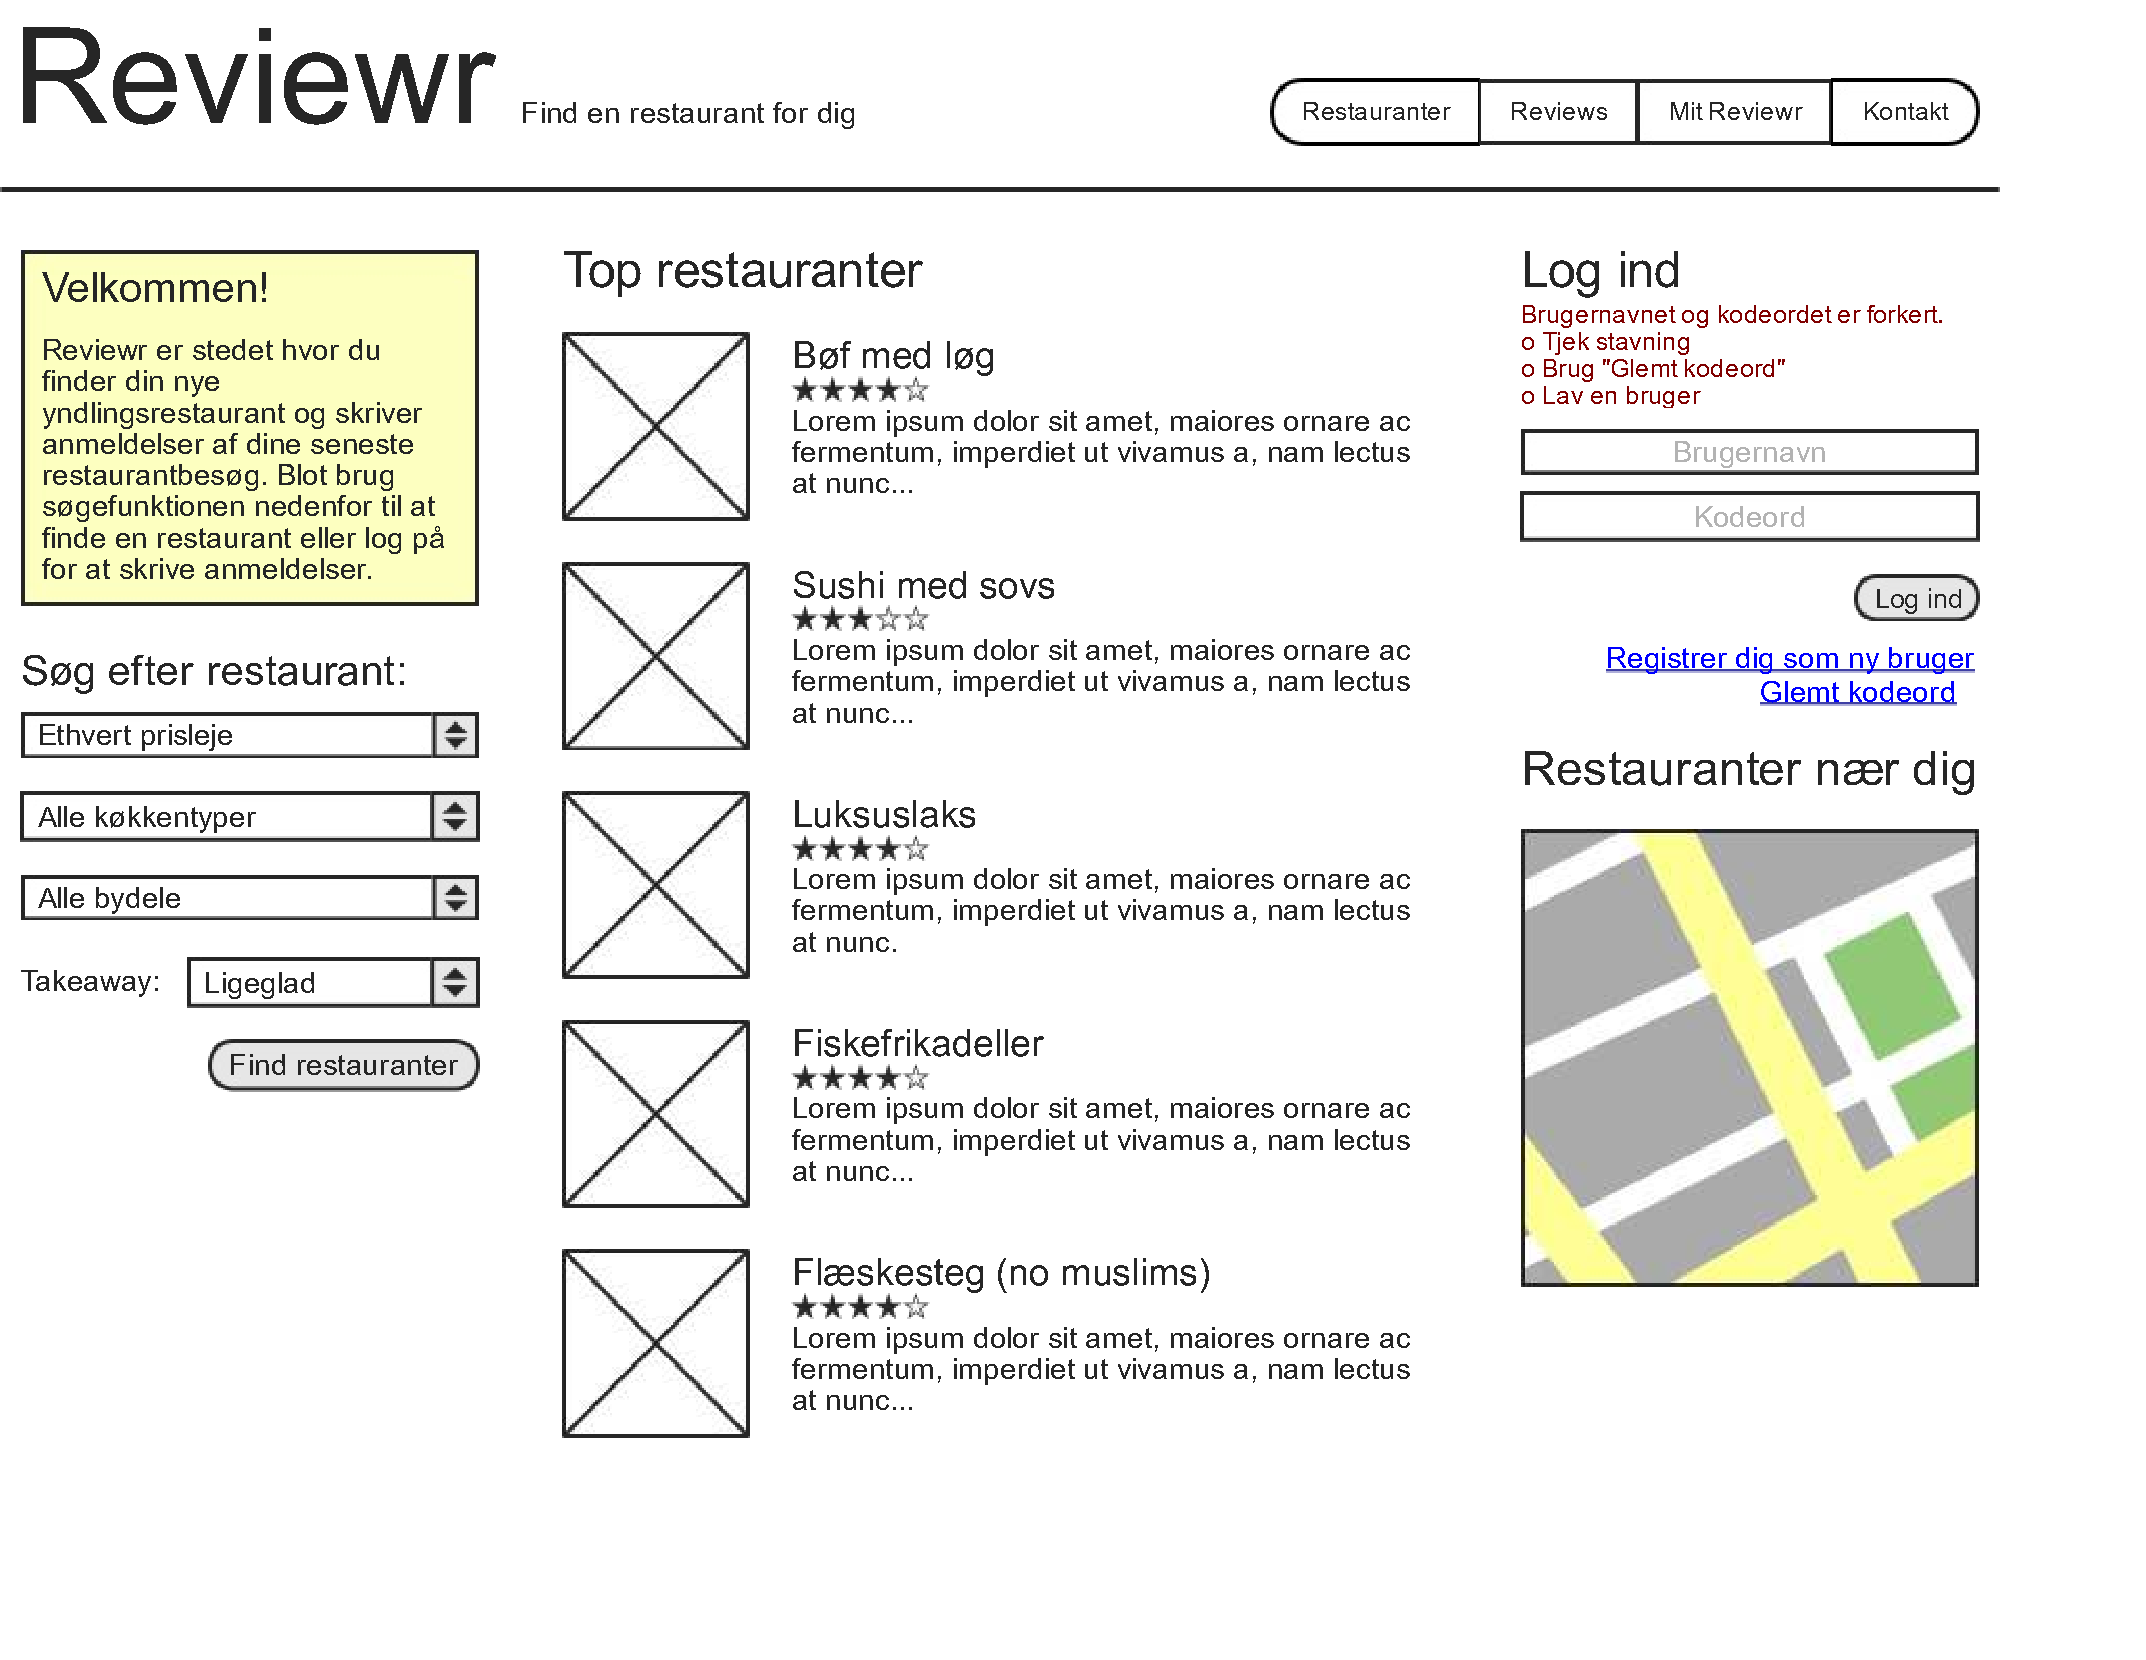
\includegraphics[width=0.9\textwidth]{mockup/page4.pdf}
  \caption{Forsiden med en fejlmeddelelse fordi brugeren har indtastet
    forkert brugernavn eller løsen.}
\end{figure}

\begin{figure}[hp]
  \centering
  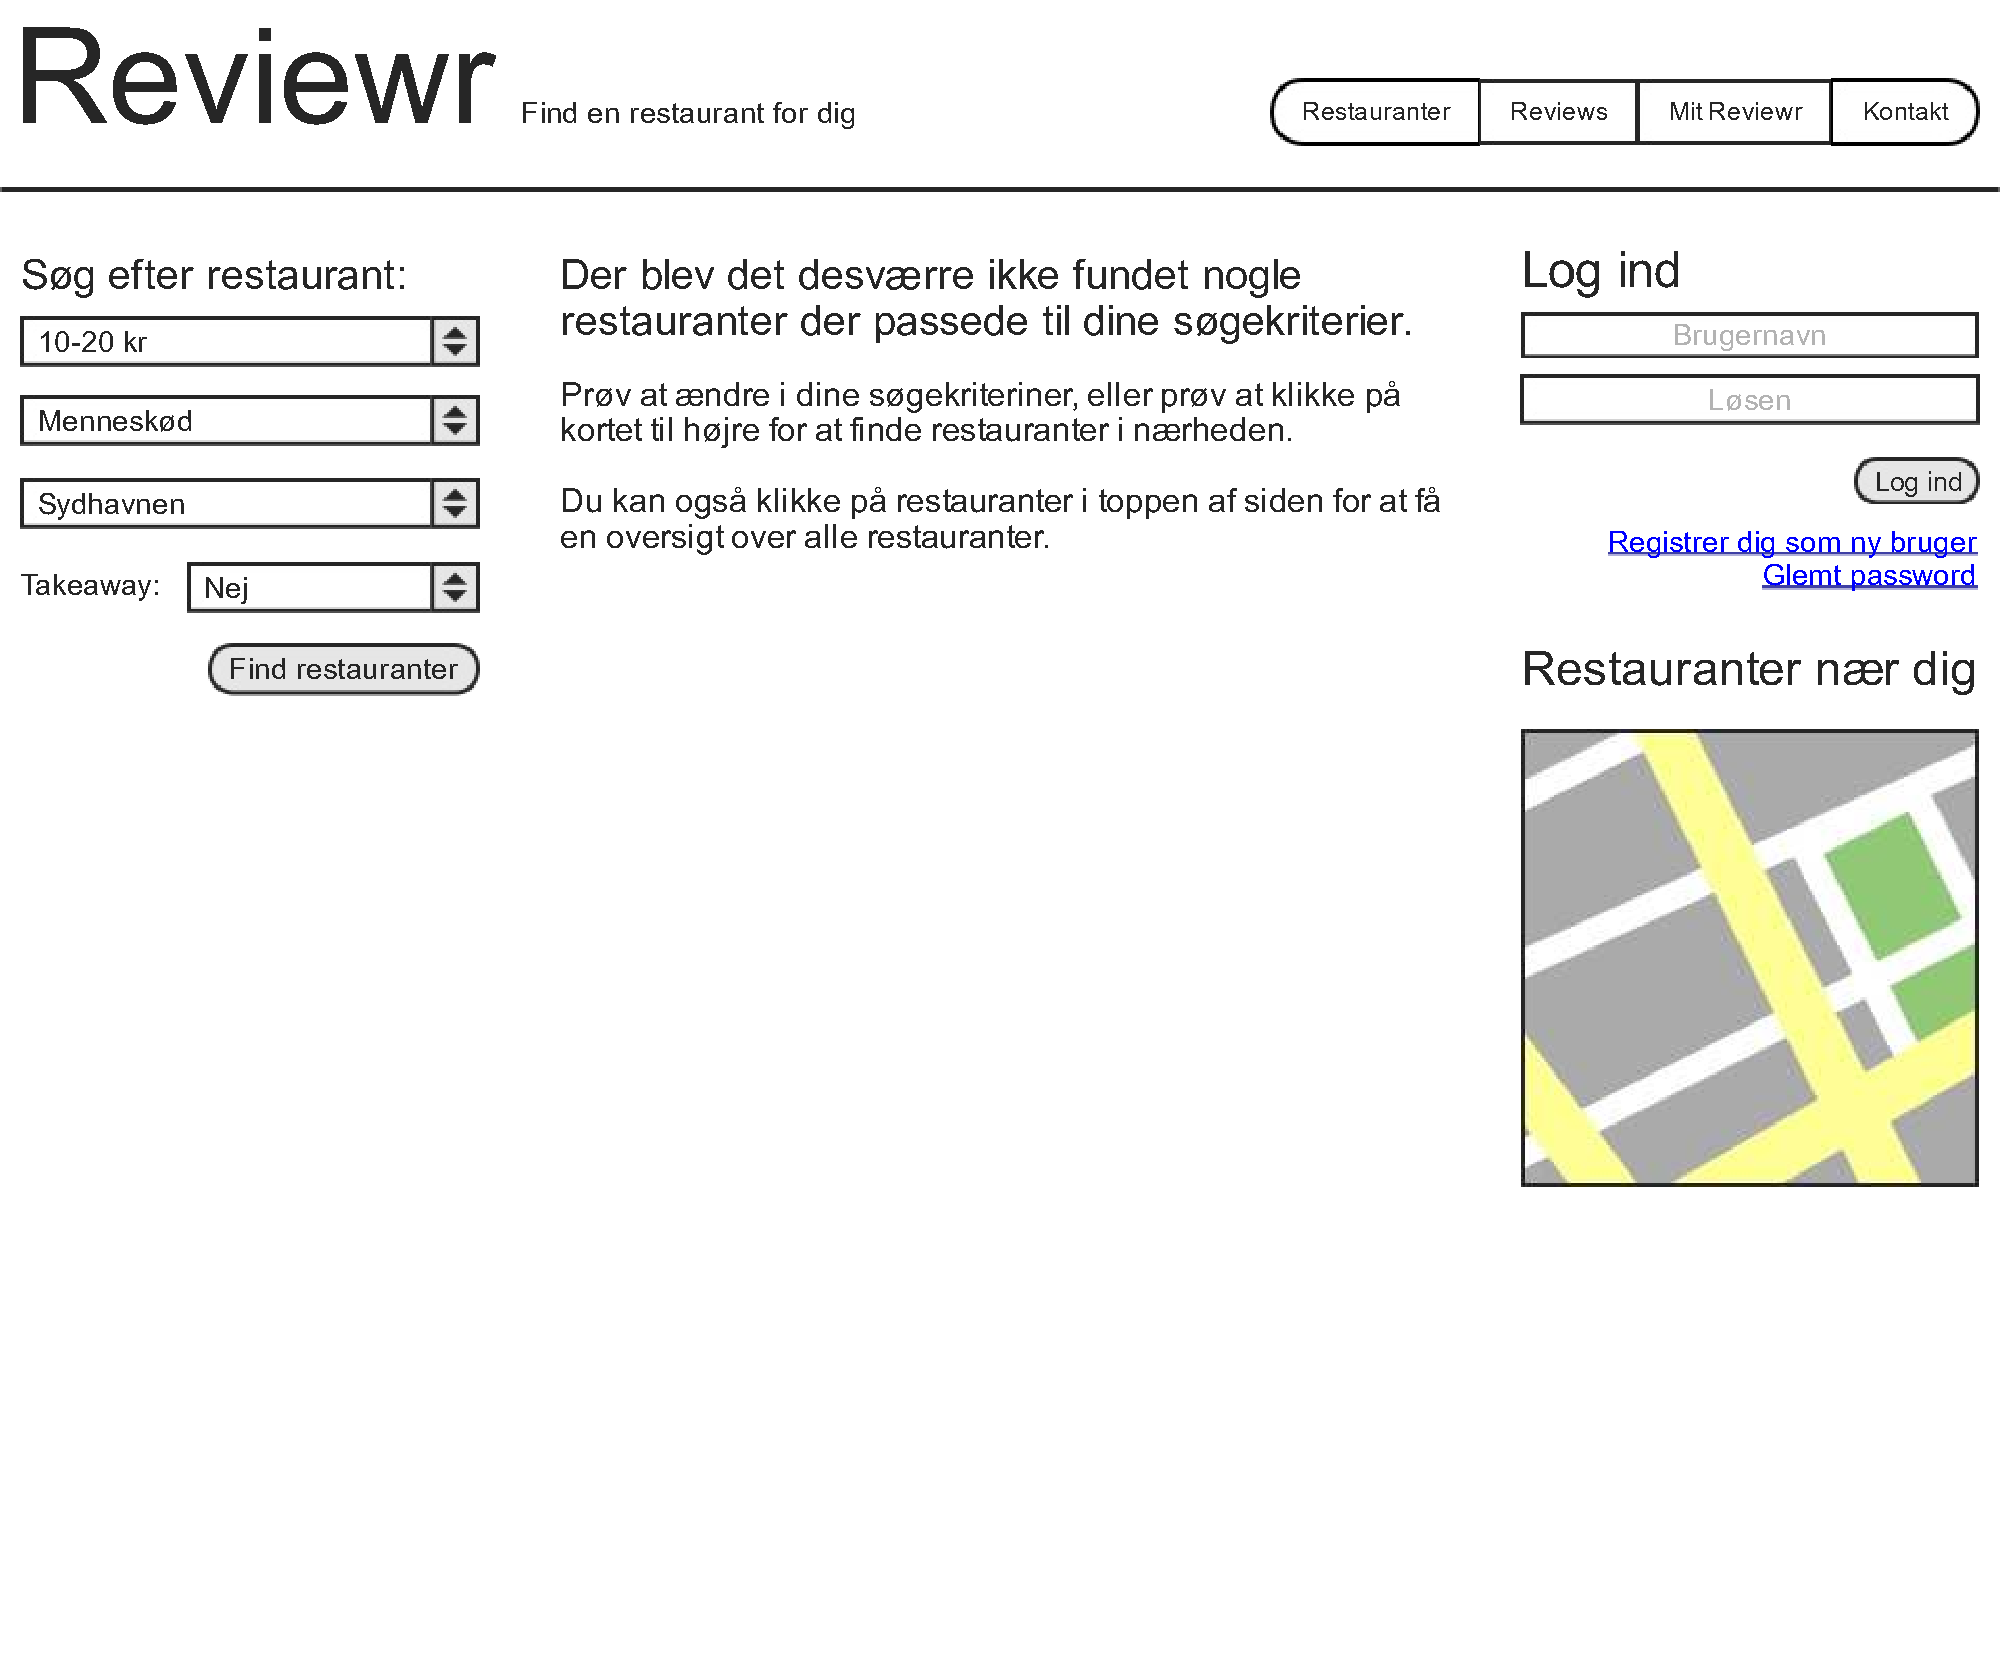
\includegraphics[width=0.9\textwidth]{mockup/page5.pdf}
  \caption{Siden der vises når søgningen returnerer nul resultater.}
\end{figure}


\printbibliography[heading=bibnumbered,title=Litteraturliste]

\end{document}
